% !TeX spellcheck = en_US
\documentclass[10pt,a4paper,titlepage]{article}
\usepackage[utf8]{inputenc}
\usepackage[T1]{fontenc}
\usepackage{amsmath}
\usepackage{amsfonts}
\usepackage{amssymb}
\usepackage{makeidx}
\usepackage{graphicx}
\usepackage[left=2.00cm, right=2.00cm, top=2.00cm, bottom=2.00cm]{geometry}
\usepackage{tikz}
\usepackage{tikz-uml}
\usepackage{wallpaper}
\linespread{1}
\usetikzlibrary{patterns}%for tikz https://tex.stackexchange.com/questions/54464/hatch-a-rectangle-in-tikz
%sources
\usepackage[backend=bibtex,style=alphabetic]{biblatex}
\bibliography{Thesis}
%Makes index browsable in pdf viewers and shows index in sidebar
\usepackage[bookmarks]{hyperref}
%Captions for figures in minipage
\usepackage{caption}

%\author{Mikail Gedik}
%Ensures that \ref works with paragraphfs as intended
\setcounter{secnumdepth}{6}

%For svg images in subdirectory
\graphicspath{{res/images/}}

\begin{document}	
	\begin{titlepage}
		\ThisCenterWallPaper{1}{"./res/images/titleImageReworked.jpeg"}
		\null
		\newpage
	\end{titlepage}
	
	\pagenumbering{roman}
	\tableofcontents
	\listoffigures
	\clearpage
	\pagenumbering{arabic}
	\let\oldref\ref
	\renewcommand{\ref}[1]{\oldref{#1} (page~\pageref{#1})}
	
	\section{Abstract}
	This paper describes the coding of a program in Java and OpenCL capable of calculating a few selected fractals and casts light on the core aspects I have implemented, such as how the data is calculated and stored. The paper will first explain what a fractal is, albeit only briefly since they do not have to be discussed in depth for my use case. The next section \ref{sec:fractals} shortly describes the functionalities and the structure of my program, breaking it down into logical components depending what they are responsible for. The last section is dedicated to bugs, known issues and their workarounds, limitations and possible ways of improving of my program, followed by a reflection on my work.
	\section{What are Fractals?}\label{sec:fractals}
	Mathematicians used to rely exclusively on classical algebra to describe as well as research sets and functions. As classical algebra is only able to describe regular sets and functions, any irregular set could not by described and ended up being labeled as pathological, irrelevant and not being paid any further attention. This decision however was found to be a fallacy, as irregular functions and sets provide a better representation of natural phenomenons and structures (for example coast lines, cloud borders, turbulence in fluids, snow flakes (see figure \ref{fig:snowflake})) than normal shapes described by classical geometry. These irregular sets and functions are now known as fractals. 
	While they were first conceptualized by Felix Hausdorff in 1918, it was only in the 1970s, after the advent of computers with their impressive computational power, that the exploration of fractals became much easier. The term fractal (from Latin \emph{fragmented, broken}) ) was coined in 1975 by mathematician Benoît B. Mandelbrot. Mandelbrot used fractals as a tool to examine the stock market, but they have proved to be useful in various fields like physical chemistry, fluid mechanics and physiology \cite{FalconerKennethJ1993FG:m, britannica}.
	\subsection{The Sierpiński Triangle}
	The properties of fractals will be illustrated utilizing with the aid of the Sierpiński triangle (figure \ref{fig:sierpinski_triangle}). The structure, while seeming complex at first glance, reveals a rather simple creation process. As illustrated in figure \ref{fig:sierpinski_triangle_build} the construction starts with a filled triangle which is split into three smaller triangles by cutting out an triangular upside-down hole. The resulting triangles are once again cut out, creating more triangles. This process is repeated \emph{ad infinitum} on any newly created triangles. \\
	The first notable property is the perfect self similarity. An infinite amount of scaled down copies of the fractal can be found in the original structure. This property is also found in other fractals, including the Mandelbrot or Julia set, although the copies often only resemble the original approximately. Some fractals display a statistical self similarity, meaning that the copies statistically show the same properties at many scales.\\
	The next property is indirectly a predecessor of the aforementioned self similarity. Fractals have to contain a certain microstructure. The Sierpiński triangle can be magnified infinitely without ever showing a final structure which is not fractured itself. Additionally, the local geometry cannot be described by classical Euclidean (meaning shapes like circles, lines, spheres, cuboids and such) geometry; the structure is by far not adequately regular.\\
	Contrary to its appearance, the definition of the Sierpiński triangle is thus quite simple. Furthermore, it is a recursive. Both these properties are often also characteristic of other fractals.\\
	Although it lies outside the scope of this paper, the Hausdorff dimension is also worth mentioning. Broadly speaking, the Hausdorff dimension is a real number (as opposed to the topological dimensions, which are always integers) which describes how much space a set fills up and it is usually greater than its topological dimension \cite[Einleitung]{FalconerKennethJ1993FG:m}.
	
	\begin{figure}[h]
		\caption{Sierpiński triangle \cite{sierpinski_image}}
		\label{fig:sierpinski_triangle}
		\centering
		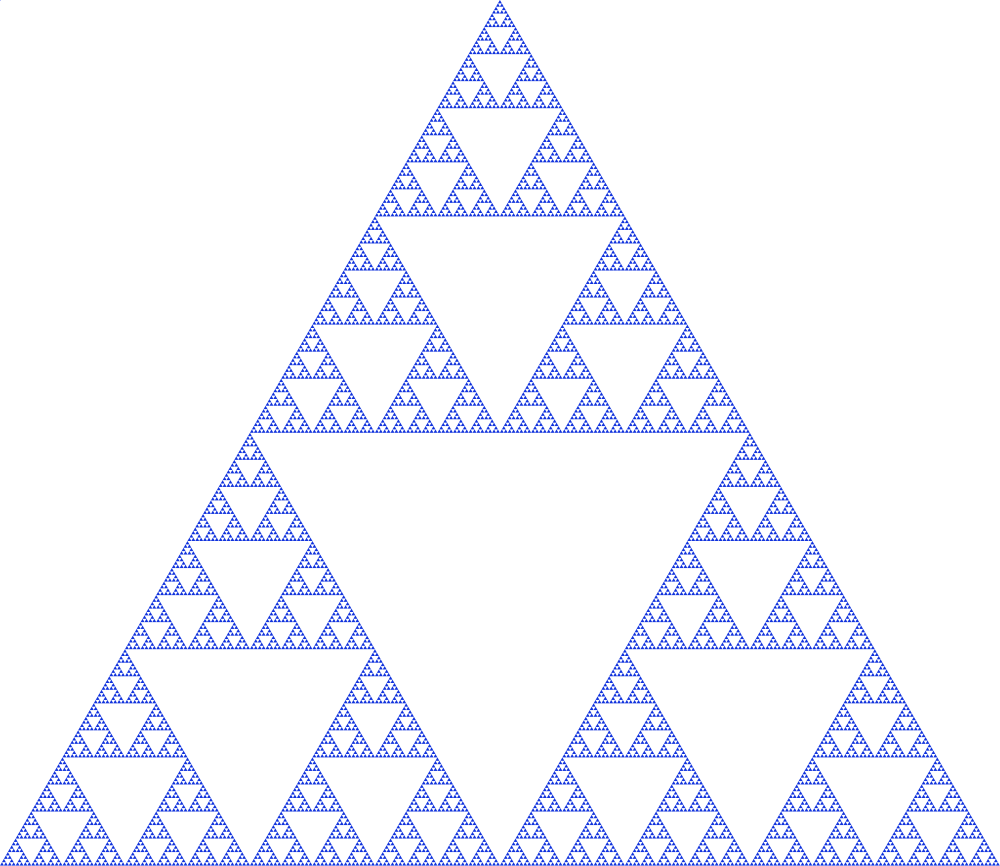
\includegraphics[width=0.5\textwidth]{"res/images/1000px-Sierpinski_triangle.svg.png"}
	\end{figure}
	\begin{figure}[h]
		\caption{Each branch of the snowflake creates new smaller branches \cite{wikipedia_snowflake}}
		\label{fig:snowflake}
		\centering
		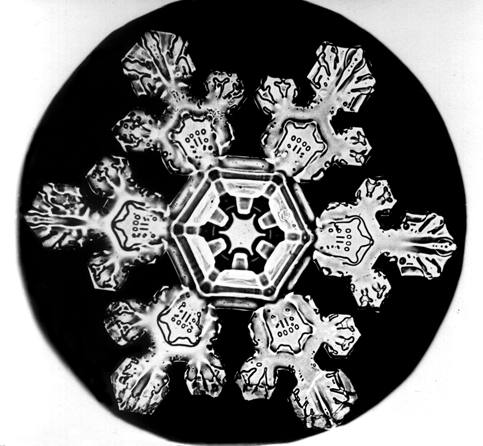
\includegraphics[width=0.5\textwidth]{"res/images/bentley_snowflake.jpg"}
	\end{figure}
	\begin{figure}[h]
		\caption{Creation of the Sierpinski triangle}
		\label{fig:sierpinski_triangle_build}
		\centering
		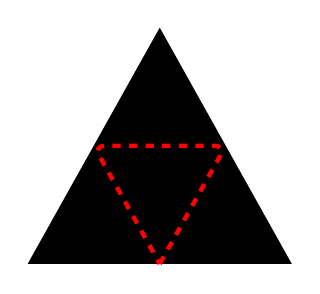
\begin{tikzpicture}[scale=3]
		\fill[black] (0,0) -- (1.118,0) -- (1.118/2, 1);
		
		\draw[rounded corners, dashed, red, ultra thick] (1.118/2, 0) -- (1.118/4*3,.5) -- (1.118/4, .5) -- (1.118/2, 0);
		\end{tikzpicture}
		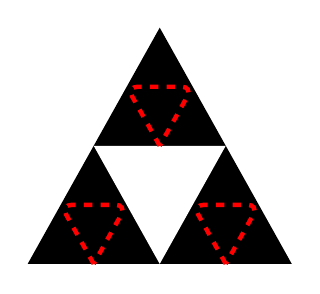
\begin{tikzpicture}[scale=3]
		\fill[black] (0,0) -- (1.118033989,0) -- (1.118033989/2, 1);
		\fill[white] (1.118/2, 0) -- (1.118/4*3,.5) -- (1.118/4, .5);
		
		\draw[rounded corners, dashed, red, ultra thick] (1.118/4*3, 0) -- (1.118/8*5,.25) -- (1.118/8*7, .25) -- (1.118/4*3, 0);
		\draw[rounded corners, dashed, red, ultra thick] (1.118/4, 0) -- (1.118/8,.25) -- (1.118/8*3, .25) -- (1.118/4, 0);
		\draw[rounded corners, dashed, red, ultra thick] (1.118/2, .5) -- (1.118/8*3,.75) -- (1.118/8*5, .75) -- (1.118/2, .5);
		\end{tikzpicture}
		
\begin{tikzpicture}[scale=3]
		\fill[black] (0,0) -- (1.118033989,0) -- (1.118033989/2, 1);
		
		\fill[white] (1.118/2, 0) -- (1.118/4*3,.5) -- (1.118/4, .5);
		
		\fill[white] (1.118/4*3, 0) -- (1.118/8*5,.25) -- (1.118/8*7, .25);
		\fill[white] (1.118/4, 0) -- (1.118/8,.25) -- (1.118/8*3, .25);
		\fill[white] (1.118/2, .5) -- (1.118/8*3,.75) -- (1.118/8*5, .75);
		\end{tikzpicture}
	\end{figure}
	
	\subsection{The Mandelbrot Set}
	Although most of my senior thesis revolves around computer science the necessity arises to explain the fractal crucial in my work. The Mandelbrot set was named after Benoît B. Mandelbrot, and is the first one to be called a fractal. In terms of properties, it is related to the Julia set, which is also not a part of my work, although my program has the ability to display it. The Mandelbrot set \(\mathbb{M}\) is an, unlike the previously mentioned geometric Sierpiński triangle, the Mandelbrot set \(\mathbb{M}\) is an algebraic fractal in the complex plane \(\mathbb{C}\). There are multiple definitions for the set, but the most relevant for my work is as follows:
	\begin{align*}
			f_{c}(z)&=z^2 + c\\
			f_{c}^{n} &= f_{c} \circ f_{c} \dots \circ f_{c}\\
			\mathbb{M} &= \{c \in \mathbb{C}: f_{c}^{n}(0)\not\to\infty \text{ for } n \to \infty\}
	\end{align*}
	Each point \(c \in \mathbb{C}\) has a corresponding function \(f_c(z)=z^2 +c\). Now let \(z_0=0\), \(z_1 = f_c(z_0)\), \(z_2 = f_c(f_c(z_0))\), or more generally \(z_n = f_c(f_c(\dots f_c(0)))= f_c^n(0)\). The example below may be more easily understood with the recursive definition \(z_{n+1}=z_n^2+c\). \(z_k\) is called the \(k\)th iteration of a point. If \(|z_n|\) grows to infinity for \(n \to \infty\), \(c\) is not part of the set. On the other hand, if \(|z_n|\) tends to a finite number, \(c\) is part of the set.\\
	Table \ref{fig:iterations_mandelbrot} shows the first ten iterations of two examples. It is trivial that \(z_1=c\), since \(z_0 = 0\). While \(z_n\) diverges quickly for \(c=0.9 - 0.2i\), it remains small and does not tend to infinity for \(c=0.3+0.2i\). For any other \(c\) it may take hundreds of thousand of iterations to diverge. Whilst no proof will be provided, since it lies outside the scope of this paper, it can be shown that \(\lim_{n\to\infty}z_{n} = \infty\) if \(|z_{k}| > 2\) for any \(k\), meaning that further iterations are not necessary to determine that a point is not part of the set. Theoretically, a point has to go through an infinite amount of iterations to prove that it is part of the set and does not diverge. To complete this obviously unaccomplishable task, programs usually only calculate a limited amount of iterations and give up as soon as that maximum is reached. Raising the limit creates more detail in the fractal at the cost of calculation time, but this is only necessary when magnifying the set \cite[Chapter 14.2]{FalconerKennethJ1993FG:m}.
	\begin{figure}
		\centering
		\caption{Iterations of different \(c\)}
		\label{fig:iterations_mandelbrot}
		\begin{minipage}{.45\textwidth}
			\centering
			\begin{tabular}{c|l}
				\multicolumn{2}{c}{\(c=0.3+0.2i\)} \\ \hline
				\(z_1\)& \(0.3\, -0.2 i\)\\ \hline
				\(z_2\)& \(0.35\, -0.32 i\)\\ \hline
				\(z_3\)& \(0.3201\, -0.424 i\)\\ \hline
				\(z_4\)& \(0.222688\, -0.471445 i\)\\ \hline
				\(z_5\)& \(0.12733\, -0.40997 i\)\\ \hline
				\(z_6\)& \(0.148137\, -0.304403 i\)\\ \hline
				\(z_7\)& \(0.229284\, -0.290187 i\)\\ \hline
				\(z_8\)& \(0.268363\, -0.33307 i \)\\ \hline
			\end{tabular}
		\end{minipage}
		\begin{minipage}{.45\textwidth}
			\centering
			\begin{tabular}{c|l}
				\multicolumn{2}{c}{\(c=0.9-0.2i\)} \\ \hline
				\(z_1\)& \(0.9\, + 0.2 i\)            \\ \hline
				\(z_2\)& \(1.67\, +0.56 i\)            \\ \hline
				\(z_3\)& \(3.3753\, +2.0704 i\)           \\ \hline
				\(z_4\)& \(8.00609\, +14.1764 i\)            \\ \hline
				\(z_5\)& \(-135.974+227.196 i\)            \\ \hline
				\(z_6\)& \(-33128.1-61785.2 i\) \\ \hline
				\(z_7\)& \(-2.71994\times 10^9+4.09366\times 10^9 i\)           \\ \hline
				\(z_8\)& \(-9.35996\times 10^{18}-2.2269\times 10^{19} i\) \\ \hline
			\end{tabular}
		\end{minipage}
	\end{figure}
	\begin{figure}
		\caption{The Mandelbrot set}
		\label{fig:mandelbrot}
		\centering
		
\includegraphics[width=0.5\textwidth]{"res/images/mandelbrot.png"}
	\end{figure}
	\section{The Program}
	This section represents the core of my paper. It starts by listing the capabilities of my program without giving technical details to the underlying model, which in turn is described as next. Lastly, the implementation is discussed.
	\subsection{Program Functionalities}
	My program is able to calculate and render fractals. Before starting the calculation engine, parameters of the calculation can be set, for example the maximal amount of iterations a point can go through before assuming that it is part of the Mandelbrot set. Once the render engine has been started, the user can move around and zoom into the fractal. Should an interesting spot be identified, the user can export the location as an image and save it to the disk. It is also possible to create an animation and export it as a video. The export dialog offers the option to change the resolution. The raw calculation data may also be saved to, or loaded from, the disk.\\
	Users familiar with OpenCL can also modify the calculation and render kernel in order to change the fractal and coloring function. Depending on how many iterations are requested by the user massive computing power is needed. Should the local power not suffice to achieve the result in useful time, it is possible to harness the computing power of multiple computers by connecting them to each other. One machine then acts as the ``master'' and coordinates all the other machines (``slaves''), while they in turn calculate the fractal.
	
	%TODO SVG images
	\iffalse	
	\begin{figure}
		\centering
		\def\svgwidth{0.5\textwidth}
		\input{res/images/units_chain.pdf_tex}
	\end{figure}
	\fi
	
	\subsection{Structure}
	Programs are usually programmed in a divide-and-conquer manner. Instead of implementing the project as a whole, it is split in smaller non autonomous sub modules. This has several advantages. Because the code is grouped in smaller modules, the project is easier to maintain over time as specific pieces of code can be found easier when the need to edit them arises. Also, other coders will understand the code better if it is structured practically.\\
	Another perk is the ease of debugging. The modules are like links tied together in a chain. When the program has to do something, the first link receives an order to do what it was programmed to and passes an interim result to the next link, which does another calculation composing a new interim result. This process is repeated until the end of the chain is reached where the final result is created. A single faulty link out of thousands will likely screw up the entire procedure. The search for the culprit, alias debugging, is much easier when the code is not written in a single big block, because the interim results can be inspected, betraying any faulty links. It is also possible to test a single modules (unit testing) instead of the whole program.\\
	Figure \ref{fig:program_structure} shows how the code is grouped and structured in smaller components, as well as how they interact with each other. The harshest division is between the core, which encapsulates the logic to calculate, store and render data, and the GUI (graphical user interface) which offers a window for the user to interact with. This is because a programmer may wish to use the calculation capabilities in his own program and no GUI is needed. This way the GUI can be easily omitted.\\
	The next section will only briefly describe how the single modules work, starting with the core components and then moving on to the less complex GUI. An in-depth discussion will follow in section \ref{sec:implementation}.
	\begin{figure}
		\centering
		\caption{Program structure}
		\label{fig:program_structure}
		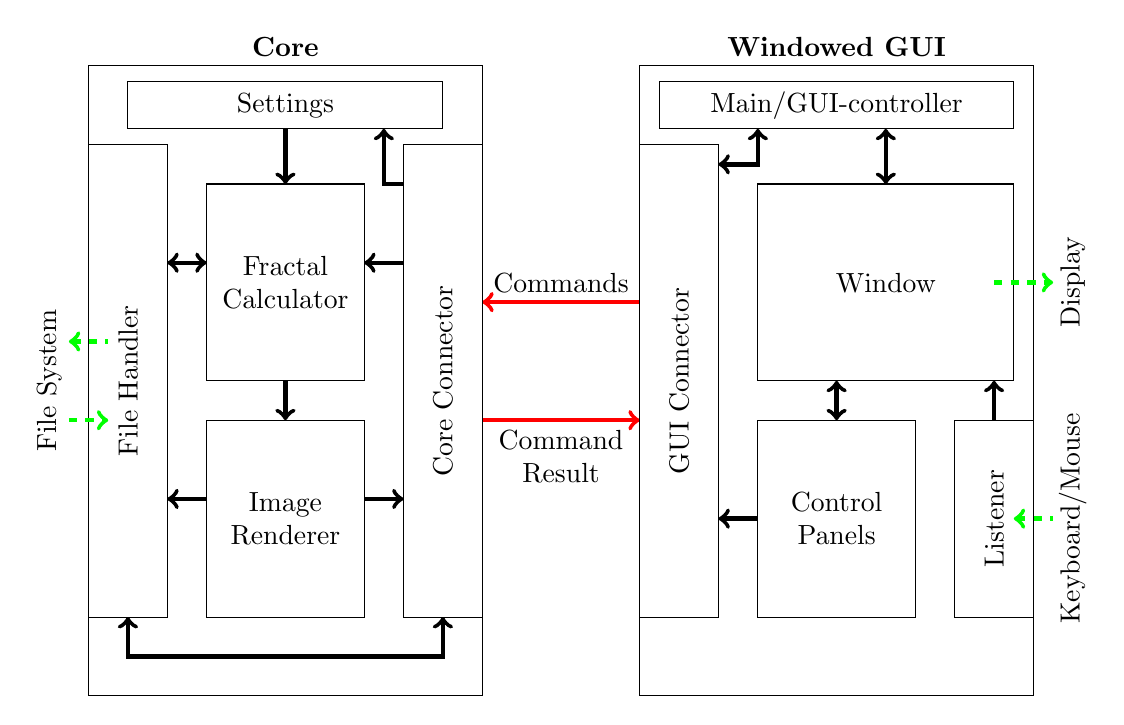
\begin{tikzpicture}
		%Front/Backend-connection
		\draw[red, ultra thick, <-] (5,5) -- (7,5);
		\node[above, align=center] at (6,5) {Commands};
		
		\draw[red, ultra thick, ->] (5,3.5) -- (7,3.5);
		\node[below, align=center] at (6,3.5) {Command\\Result};
		
		%Backend
		\draw (0,0) rectangle (5,8);
		\node[above] at (2.5, 8) {\textbf{Core}};
		
		%Interface
		\draw (4,1) rectangle (5, 7);
		\node[rotate = 90] at(4.5, 4) {Core Connector};
		
		%Settings
		\draw (.5,7.2) rectangle (4.5, 7.8);
		\node at (2.5, 7.5) {Settings};
		
		%Fractal calculator
		\draw (1.5,4) rectangle (3.5, 6.5);
		\node[align=center] at (2.5, 5.25) {Fractal\\Calculator};
		
		%Image render
		\draw (1.5,1) rectangle (3.5, 3.5);
		\node[align=center] at (2.5, 2.25) {Image\\Renderer};
		
		%File handling
		\draw (0,1) rectangle (1, 7);
		\node[rotate = 90] at(.5, 4) {File Handler};
		
		%Arrows
		%Settings-Frac
		\draw[ultra thick, ->] (2.5, 7.2) -- (2.5, 6.5);
		%Int-Frac
		\draw[ultra thick, <-] (3.5, 5.5) -- (4, 5.5);
		%Frac-Image
		\draw[ultra thick, ->]  (2.5, 4) -- (2.5, 3.5);
		%Img-Int
		\draw[ultra thick, ->]  (3.5, 2.5) -- (4, 2.5);
		%Frac-File
		\draw[ultra thick, <->] (1.5, 5.5) -- (1, 5.5);
		%Image-File
		\draw[ultra thick, ->] (1.5, 2.5) -- (1, 2.5);
		%Settings-Int
		\draw[ultra thick, ->] (4, 6.5) -- (3.75, 6.5) -- (3.75, 7.2); 
		%Int-File
		\draw[ultra thick, <->] (4.5, 1) -- (4.5,.5) -- (.5,.5) -- (.5, 1);
		
		%File system
		\draw[green, ultra thick, dashed, ->] (-.25, 3.5) -- (.25, 3.5);
		\draw[green, ultra thick, dashed, <-] (-.25, 4.5) -- (.25, 4.5);
		\node[rotate = 90] at (-.5, 4) {File System};
		
		%Frontend
		\draw (7,0) rectangle (12,8);
		\node[above] at (9.5, 8) {\textbf{Windowed GUI}};
		
		%Interface
		\draw (7,1) rectangle (8, 7);
		\node[rotate = 90] at(7.5, 4) {GUI Connector};
		
		%Main
		\draw (7.25,7.2) rectangle (11.75, 7.8);
		\node at (9.5, 7.5) {Main/GUI-controller};
		
		%Window
		\draw (8.5,4) rectangle (11.75, 6.5);
		\node[align=center] at (10.125, 5.25) {Window};
		
		%Control Panels
		\draw (8.5,1) rectangle (10.5, 3.5);
		\node[align=center] at (9.5, 2.25) {Control\\Panels};
		
		%Listener
		\draw (11,1) rectangle (12, 3.5);
		\node[rotate = 90] at(11.5, 2.25) {Listener};
		
		%Arrows
		%Main-Win
		\draw[ultra thick, <->] (10.125 ,7.2) -- (10.125, 6.5);
		%List-Win
		\draw[ultra thick, ->] (11.5, 3.5) -- (11.5,4);
		%Ctr-Win
		\draw[ultra thick, <->] (9.5, 3.5) -- (9.5, 4);
		%Main-Interface
		\draw[ultra thick, <->] (8, 6.75) -- (8.5, 6.75) -- (8.5, 7.2);
		
		%Ctr-Interface
		\draw[ultra thick, <-] (8, 2.25) -- (8.5, 2.25);
		
		%Keyboard/Mouse
		\draw[green, ultra thick, dashed, ->] (11.5, 5.25) -- (12.25,5.25);
		\node[rotate = 90] at (12.5, 5.25) {Display};
		
		\draw[green, ultra thick, dashed, <-] (11.75, 2.25) -- (12.25, 2.25);
		\node[rotate = 90] at (12.5, 2.25) {Keyboard/Mouse};
		\end{tikzpicture}
	\end{figure}
	
	\subsubsection{Core}
	The core consists of multiple components or units, which are tightly bound together. Each of them is responsible for a certain task and should not do anything else. The modules are capable of communicating to the connector, and in some cases each other, but are isolated from the ``outside'', with the exception of the connector and file handler. These two interchange data with either the UI or the underlying file system.
	\paragraph{Settings}
	The settings are configurations used either directly during computation or as parameters for the program itself. Variables used during the computation could be for example the maximal number of iterations allowed  or the color function used when rendering the data. The settings can only be changed before the actual fractal calculator is started.
	\paragraph{Database}
	The data model is the one of the most complex parts of my project, as the data has to have low access times to lots of data. To achieve this, the data is logically split multiple times. The topmost containers are called levels and sort the data by precision (more to that in section \ref{sec:implementation}). They do not contain the data directly but instead are made up by clusters, which store small chunks of data sorted by location. The size of these chunks is determined by the settings.
	\paragraph{Fractal Calculator}
	The calculator determines if points are part of the set, and if not how many iterations it takes to be sure that the point is not in the set. It contains the logic to harness the power graphic cards provide using OpenCL and can even connect to other computers to use their computing power as well.
	\paragraph{Renderer}
	The renderer converts raw data to an image. The amount of iterations a point has gone through before it escaped the set is mapped to a specific color depending on the color function defined.
	\paragraph{Connector}
	The connector conduces all the components and provides the API to control the core, meaning that the GUI can issue commands only through the connector. This adds an extra level of abstraction, as the GUI does not have to worry about how the core calculates data and only has to request an image. 
	\subsubsection{GUI}
	The GUI is the face my program has when utilized. Although most of my efforts have gone towards developing the core, a stable GUI still had to be developed. The application consists of a simple main window and an occasional popup when user input such selecting a file is required.
	\paragraph{Login}
	Upon starting the application, a login screen is displayed. The user can adjust the settings by opening the settings dialog and edit the calculation and render kernel if he has the knowledge to. It is also possible to start the application as a slave.\\
	When the start button is pressed, the user can select which computer parts are used to render the fractal. Usually, only installed GPUs will show up as an option, but machines with OpenCL support on the CPU will also show a CPU. If the program accepts external slaves they will also show up as options. After confirming the selection the program changes to the master view. If the slave option was selected, the program attempts to connect to the specified master and shows the slave view, which is empty.
	\paragraph{Master View}
	The master view consists of the fractal in the middle and a menu bar on top containing entries to export images or videos and save calculated data. By left clicking and dragging the mouse the user is able to move around. Dragging using the right mouse button selects an area which will be magnified. It is also possible to zoom using the mouse wheel. Alternatively, the viewport can also changed via the menu bar.
	\subsection{Implementation}\label{sec:implementation}
	This section discusses the functionalities in greater depth, although without going into the Java specific implementations, i.e. no classes or class methods will be mentioned.
	\subsubsection{Core}
	\paragraph{Dataset}
	The connector passes the data generated from the calculator to the dataset where it is stored. The data consists of points (or mathematically speaking complex numbers) which each have a value corresponding to the amount of iterations the program has applied to a point. To facilitate further use, the point and its value are from now on grouped in a structure called entry. Table \ref{fig:entries} shows three entries with values. The \(-1\) denotes that the point did not diverge and is thus in the Mandelbrot set.
	\begin{figure}
		\centering
		\caption{A table containing entries}
		\label{fig:entries}
		\begin{tabular}{c|c}
			Point        & Value \\ \hline
			\(0.3+0.3i\) & -1    \\ \hline
			\(0.4+0.2i\) & 31    \\ \hline
			\(0.4+0.5i\) & 7     \\
		\end{tabular}
	\end{figure}
	\subparagraph{General Understanding}
	\begin{figure}
		\caption{Schematic of the dataset}
		\label{fig:dataset_schematic}
		\centering
		\def\svgwidth{\textwidth}
		\input{res/images/dataset.pdf_tex}
	\end{figure}
	This section gives an insight on how the data is sorted in the dataset without going into mathematical details, which will done in the following sections \ref{sec:clusters} and \ref{sec:levels}. Figure \ref{fig:dataset} and \ref{fig:dataset_schematic} illustrates the separation of points of the set (green) into clusters (red) and levels (blue). The topmost square shows the entire ``raw'' dataset and the three following squares each show a level with clusters.\\
	To understand the model further the purpose of the data has to be considered, which is generating images. Broadly speaking, every pixel represents a point in the dataset. Because all pixels have the same distance to their neighboring pixels all points needed have the same distance to their neighboring points. It is thus sensible to sort points by their distance to their neighbors. This makes it possible to quickly query the necessary points when an image is rendered instead of having to search the entire dataset. This is put to practice by the so called levels.\\
	Furthermore, the image often only shows a part of the area the dataset spans over, meaning that only the points in that part of the area are needed. The image creation process will thus mostly need a subset of the points. Since the points needed are also always close to each other, it makes sense to group the points by their location in small chunks, called clusters in my program. Their advantage is that they can be queried much faster than single values.\\	
	Another notable thing is that the data in the set is not randomly distributed but presented in a raster. The dataset requires that data added fits into the present structure. The reasoning behind this is explained more thoroughly in section \ref{TODO}.\\
	Every cluster contains exactly four points, regardless of the level it is in. The size however is given by the level.
	\begin{figure}
		\centering
		\caption{An exemplary dataset with \(L_0\) to \(L_2\)}
		\label{fig:dataset}
		\begin{minipage}{.4\textwidth}
			\centering
			\begin{tikzpicture}
			\node at (2,2) {
\includegraphics[width=4cm, height=4cm]{res/images/mandelbrot.png}};
			\draw[ultra thick] (0,0) rectangle (4,4);
			\foreach \x in {0,...,15} {
				\foreach \y in {0,...,15}{
					\fill[green] (.25 * \x + .125, .25 * \y + .125) circle[radius=.05];
				}	
			}
			\end{tikzpicture}
		\end{minipage}\\
		\begin{minipage}{.4\textwidth}
			\centering
			\begin{tikzpicture}
			\node at (2,2) {
\includegraphics[width=4cm, height=4cm]{res/images/mandelbrot.png}};
			\draw[ultra thick, blue] (0,0) rectangle (4,4);
			\draw[step=2,red, dashed] (0,0) grid (4,4);
			\foreach \x in {0,...,3} {
				\foreach \y in {0,...,3}{
					\fill[green] (1 * \x + .5,1 * \y + .5) circle[radius=.05];
				}
			}
			\draw[red, |<->|] (0,-.2) -- (1,-.2) node[below, align = center] {\(c_{a,w}= 2\)\\\(c_{l,w}= 2\)} -- (2,-.2);
			\draw[blue, |<->|] (0,4.2) -- (2,4.2) node[above, align = center] {\(l_{a,w} = 4\)\\\(l_{l,w} = 2\)}-- (4,4.2);
			\draw[blue, |<->|] (4.2, 0) -- (4.2,2) node[right, align = center] {\(l_{a,h} = 4\)\\\(l_{l,h} = 2\)}-- (4.2,4);
			\node[right] at (3,-.8) {\(p= \frac{2}{2} = 1\)};
			\node[blue] at (-1,2) {\(L_0\)};
			\end{tikzpicture}
		\end{minipage}
		\begin{minipage}{.4\textwidth}
			\centering
			\begin{tikzpicture}
			\node at (2,2) {
\includegraphics[width=4cm, height=4cm]{res/images/mandelbrot.png}};
			\draw[ultra thick, blue] (0,0) rectangle (4,4);
			\draw[step=1,red, dashed] (0,0) grid (4,4);
			\foreach \x in {0,...,7} {
				\foreach \y in {0,...,7}{
					\fill[green] (.5 * \x + .25,.5 * \y + .25) circle[radius=.05];
				}
			}
			\draw[red, |<->|] (0,-.2) -- (.5,-.2) node[below, align = center] {\(c_{a,w}= 1\)\\\(c_{l,w}= 2\)} -- (1,-.2);
			\draw[blue, |<->|] (0,4.2) -- (2,4.2) node[above, align = center] {\(l_{a,w} = 4\)\\\(l_{l,w} = 4\)}-- (4,4.2);
			\draw[blue, |<->|] (4.2, 0) -- (4.2,2) node[right, align = center] {\(l_{a,h} = 4\)\\\(l_{l,h} = 4\)}-- (4.2,4);
			\draw[->, red] (2.5, -.2) node[below] {\(C_{2,0}=C_2\)}-- (2.5,.5);
			\draw[->, red] (4.3, 4.3) node[above right] {\(C_{3,3}=C_{15}\)}-- (3.5,3.5);
			\node[right] at (3,-.8) {\(p= \frac{1}{2} = 0.5\)};
			\node[blue] at (-1,2) {\(L_1\)};
			\draw[dashed] (-1.5, 4.5) -- (-1.5,-1.3);
			\end{tikzpicture}
		\end{minipage}\\
		\begin{minipage}{.9\textwidth}
			\centering
			\begin{tikzpicture}
				\draw[dashed] (-5,0) -- (5,0);
			\end{tikzpicture}
		\end{minipage}
		\begin{minipage}{.4\textwidth}
			\centering
			\begin{tikzpicture}
			\node at (2,2) {
\includegraphics[width=4cm, height=4cm]{res/images/mandelbrot.png}};
			\draw[ultra thick, blue] (0,0) rectangle (4,4);
			\draw[step=.5,red, dashed] (0,0) grid (4,4);
			\foreach \x in {0,...,15} {
				\foreach \y in {0,...,15}{
					\fill[green] (.25 * \x + .125, .25 * \y + .125) circle[radius=.05];
				}	
			}
			\draw[red, |<->|] (0,-.2) -- (.25,-.2) node[below,align=center] {\(c_{a,w}=0.5\)\\\(c_{l,w}= 2\)} -- (.5,-.2);
			\draw[blue, |<->|] (0,4.2) -- (2,4.2) node[above, align = center] {\(l_{a,w} = 4\)\\\(l_{l,w} = 8\)}-- (4,4.2);
			\draw[blue, |<->|] (4.2, 0) -- (4.2,2) node[right, align = center] {\(l_{a,h} = 4\)\\\(l_{l,h} = 8\)}-- (4.2,4);
			\draw[->, red] (2.25, -.2) node[below] {\(C_{4,0}=C_4\)}-- (2.25,.25);
			\draw[->, red] (4.3, 4.3) node[above right] {\(C_{15,15}=C_{63}\)}-- (3.75,3.75);
			\node[right] at (3,-.8) {\(p= \frac{0.5}{2} = 0.25\)};
			\node[blue] at (-1,2) {\(L_2\)};
			\end{tikzpicture}
		\end{minipage}
	\end{figure}

	\subparagraph{Cluster}\label{sec:clusters}
	To accelerate the querying of entries they are sorted and grouped twice, first in clusters and the in levels. The grounds to this separation are best explained using an example. Figure \ref{fig:points1} shows a complex plot containing several points on the left and a table containing the values to the right.
	\begin{figure}
		\centering
		\caption{Entries in a table}
		\label{fig:points1}
		\begin{minipage}{.4\textwidth}
			\centering
			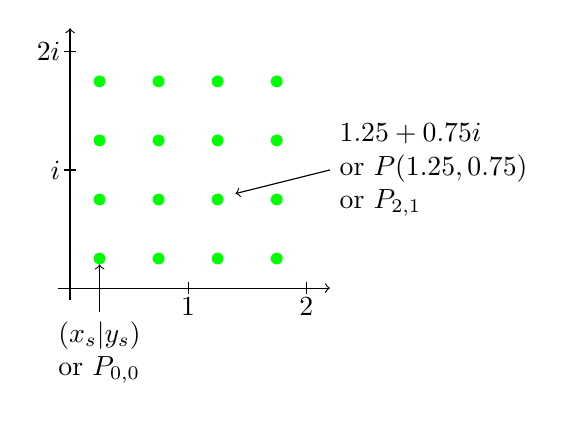
\begin{tikzpicture}[scale=1.5]
			\draw[->] (0,-.1) -- (0,1) node[left] {$i$} -- (0,2) node[left] {$2 i$} -- (0,2.2);
			\draw[->] (-.1,0) -- (1,0) node[below] {$1$} -- (2,0) node[below] {$2$} -- (2.2,0);
			\draw (-.05,1) -- (.05,1);
			\draw (-.05,2) -- (.05,2);
			\draw (1,-.05) -- (1,.05);
			\draw (2,-.05) -- (2,.05);
			
			\foreach \x in {0,1,2,3} {
				\foreach \y in {0,1,2,3}{
					\fill[green] (.5 * \x + .25,.5 * \y + .25) circle[radius=.05];
				}	
			}
			\draw[->] (2.2, 1) node[right,align=left] {\(1.25 + 0.75i\)\\or \(P(1.25,0.75)\)\\or \(P_{2,1}\)} -- (1.4, 0.8);
			\draw[->] (.25, -.2) node[below,align=left] {\((x_s|y_s)\)\\or \(P_{0,0}\)}-- (.25, .2);
			\end{tikzpicture}
		\end{minipage}
		\begin{minipage}{.4\textwidth}
			\centering
			\begin{tabular}{|c|c|}
				\hline
				Point                                  & Value \\ \hline
				\(0.25+0.25i\)                           & -1 \\ \hline
				\(0.25+0.75i\)                           & 5  \\ \hline
				\(0.25+1.25i\)                           & 2 \\ \hline
				\multicolumn{2}{|c|}{\(\dots\)} \\ \hline
				\(1.75 + 1.75i\) & 1 \\ \hline
			\end{tabular}
		\end{minipage}
	\end{figure}
	For now, each entry ``consumes'' three numbers: two floating-points for the location and an integer for the value. This can be drastically reduced by taking advantage of the fact that the points lie on an invisible grid, giving their coordinates a certain regularity. Every point's \(P_{k,j}=(x|y)\) position, where \(k\) and \(j\) stand for column and row respectively, can be described with \(x = x_s + p \times k\) and \( y = y_s + p \times j\), where \(p\) is the horizontal and vertical distance between two points, also called precision and $(x_x|y_s)$ is the first, i.e. the nearest to the lower left corner, point's position.\\
	Figure \ref{fig:points2} shows how the points are combined into the red-dashed cluster \(C\). \(c_{l,w}\) and \(c_{a,w}\) both describe the width of the cluster by different means. \(c_{l,w}\) (the \emph{logic} width) describes the amount of points the cluster contains horizontally, while \(c_{a,w}\) (the \emph{absolute} width) refers to the distance between the lower left and right corner. Additionally, the position of the cluster \((c_{a,x}|c_{a,y})\) is equal to the first points position. The attentive reader will notice that the notion implies the existence of \(c_{l,x}\) and \(c_{l,y}\), which will only be needed in section \ref{sec:levels} and are thus not yet explained.The following equations can be thus derived:
	\[c_{a,w} = p \times c_{l,w}\]
	\[c_{a,h} = p \times c_{l,h}\]
	\[\frac{c_{a,w}}{c_{l,w}} = p = \frac{c_{a,h}}{c_{l,h}}\]
	The height's derivation is not shown as it is indifferent to the width's and thus trivial. Furthermore, the total amount of points in a cluster can be calculated by \(c_{l,w} \times c_{l,h}\). To clarify the difference between the logical and absolute dimensions it may help to say that \(c_{a,w} \times c_{a,h}\) is equals to the area covered by the cluster.\\
	Using this new definitions the points' description can be further simplified. \(k\) and \(j\) can be converted into the single index \(i = k + j \times c_w\). The definitions can be summed up as the following:
	\[P_{i} = P_{(i \text{ mod } c_{l,w}), (\lfloor{i}/{c_{l,w}} \rfloor)} = (c_{a,x} + (i \text{ mod } c_{l,w}) \times p~|~c_{a,y} + (\lfloor{i}/{c_{l,w}} \rfloor) \times p)\]
	Every cluster thus has to only store it's position, the precision and an indexed list with the values. \(c_{l,w}\) and \(c_{l,h}\) are equal for all clusters in a dataset and are stored elsewhere, see section \ref{sec:levels}.
	\begin{figure}
		\centering
		\caption{The points in a cluster a list containing the values}
		\label{fig:points2}
		\begin{minipage}{.4\textwidth}
			\centering
			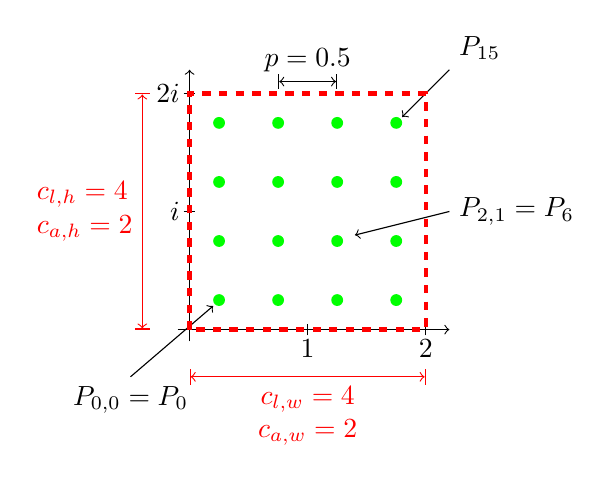
\begin{tikzpicture}[scale=1.5]
			\draw[->] (0,-.1) -- (0,1) node[left] {$i$} -- (0,2) node[left] {$2 i$} -- (0,2.2);
			\draw[->] (-.1,0) -- (1,0) node[below] {$1$} -- (2,0) node[below] {$2$} -- (2.2,0);
			\draw (-.05,1) -- (.05,1);
			\draw (-.05,2) -- (.05,2);
			\draw (1,-.05) -- (1,.05);
			\draw (2,-.05) -- (2,.05);
			
			\foreach \x in {0,1,2,3} {
				\foreach \y in {0,1,2,3}{
					\fill[green] (.5 * \x + .25,.5 * \y + .25) circle[radius=.05];
				}	
			}
			\draw[->] (2.2, 1) node[right] {\(P_{2,1} = P_{6}\)} -- (1.4, 0.8);
			\draw[->] (-.5, -.4) node[below] {\(P_{0,0} = P_{0}\)} -- (.2, .2);
			\draw[|<->|] (.75, 2.1) -- (1, 2.1) node[above] {\(p = 0.5\)} -- (1.25, 2.1);
			
			\draw[->] (2.2, 2.2) node[above right] {\(P_{15}\)}-- (1.8, 1.8);
			
			\draw[|<->|, red] (-.4,0) -- (-.4,1) node[left,align=left] {\(c_{l,h} = 4\)\\\(c_{a,h} = 2\)} -- (-.4, 2);
			\draw[|<->|, red] (0,-.4) -- (1,-.4) node[below,align=center] {\(c_{l,w} = 4\)\\\(c_{a,w} = 2\)} -- (2,-.4);
			
			\draw[red, ultra thick, dashed] (0,0) rectangle (2,2);
			\end{tikzpicture}
		\end{minipage}
		\begin{minipage}{.4\textwidth}
			\centering
			\begin{tabular}{|c|c|}
				\hline
				Index                       & Value \\ \hline
				0                           & -1 \\ \hline
				1                           & 5  \\ \hline
				2                           & 2 \\ \hline
				\multicolumn{2}{|c|}{\(\dots\)} \\ \hline
				15 & 1 \\ \hline
			\end{tabular}
		\end{minipage}
	\end{figure}
	
	\subparagraph{Levels}\label{sec:levels}
	A level \(L\) is a list of clusters which all have the same \(p\), and thus the same \(c_{a,w}\) and \(c_{a,h}\). The characteristics of levels will be described using figure \ref{fig:man_level} which contains two of them. Analogous to the clusters, the dimensions of a level can be described either by the amount of clusters the level has (\(l_{l,w},l_{l,h}\)) or the absolute dimensions \(l_{a,w},l_{a,h}\). The levels also all share their position, i.e. they overlap. The difference is that while every level shares the absolute dimensions and positions, the logical must differ. It can furthermore be inferred from the figure that \(p(L) = \frac{l_{a,w}(L)}{l_{l,w}(L) \times c_{l,w}(L)} = \frac{l_{a,h}(L)}{l_{l,h}(L) \times c_{l,h}(L)}\).
	\begin{figure}
		\centering
		\caption{The Mandelbrot in different levels}
		\label{fig:man_level}
		\begin{minipage}{.4\textwidth}
			\centering
			\begin{tikzpicture}
			\node at (2,2) {
\includegraphics[width=4cm, height=4cm]{res/images/mandelbrot.png}};
			\draw[ultra thick, blue] (0,0) rectangle (4,4);
			\draw[step=1,red, dashed] (0,0) grid (4,4);
			\foreach \x in {0,...,7} {
				\foreach \y in {0,...,7}{
					\fill[green] (.5 * \x + .25,.5 * \y + .25) circle[radius=.05];
				}
			}
			\draw[red, |<->|] (0,-.2) -- (.5,-.2) node[below, align = center] {\(c_{a,w}= 1\)\\\(c_{l,w}= 2\)} -- (1,-.2);
			\draw[blue, |<->|] (0,4.2) -- (2,4.2) node[above, align = center] {\(l_{a,w} = 4\)\\\(l_{l,w} = 4\)}-- (4,4.2);
			\draw[blue, |<->|] (4.2, 0) -- (4.2,2) node[right, align = center] {\(l_{a,h} = 4\)\\\(l_{l,h} = 4\)}-- (4.2,4);
			\draw[->, red] (2.5, -1) node[below] {\(C_{2,0}=C_2\)}-- (2.5,.5);
			\draw[->, red] (4.3, 4.3) node[above right] {\(C_{3,3}=C_{15}\)}-- (3.5,3.5);
			\node[right] at (3,-.8) {\(p= \frac{1}{2} = 0.5\)};
			\end{tikzpicture}
		\end{minipage}
		\begin{minipage}{.4\textwidth}
			\centering
			\begin{tikzpicture}
			\node at (2,2) {
\includegraphics[width=4cm, height=4cm]{res/images/mandelbrot.png}};
			\draw[ultra thick, blue] (0,0) rectangle (4,4);
			\draw[step=.5,red, dashed] (0,0) grid (4,4);
			\foreach \x in {0,...,15} {
				\foreach \y in {0,...,15}{
					\fill[green] (.25 * \x + .125, .25 * \y + .125) circle[radius=.05];
				}	
			}
			\draw[red, |<->|] (0,-.2) -- (.25,-.2) node[below,align=center] {\(c_{a,w}=0.5\)\\\(c_{l,w}= 2\)} -- (.5,-.2);
			\draw[blue, |<->|] (0,4.2) -- (2,4.2) node[above, align = center] {\(l_{a,w} = 4\)\\\(l_{l,w} = 8\)}-- (4,4.2);
			\draw[blue, |<->|] (4.2, 0) -- (4.2,2) node[right, align = center] {\(l_{a,h} = 4\)\\\(l_{l,h} = 8\)}-- (4.2,4);
			\draw[->, red] (2.25, -1) node[below] {\(C_{4,0}=C_4\)}-- (2.25,.25);
			\draw[->, red] (4.3, 4.3) node[above right] {\(C_{15,15}=C_{63}\)}-- (3.75,3.75);
			\node[right] at (3,-.8) {\(p= \frac{0.5}{2} = 0.25\)};
			\end{tikzpicture}
		\end{minipage}
	\end{figure}
	\\As new clusters are calculated they can be effortlessly be added to the levels list. This is because a level does not need to be ``complete'', i.e. clusters not needed are neither calculated nor added to the level. The values of a cluster however are always all calculated. It is not possible to calculate only half of a cluster.\\
	Since the clusters in the levels are - like the values in clusters - on a perfect grid, their position can be described by the previously mentioned \(c_{l,x}\) and \(c_{l,y}\). Similar to how \(P_{x,y}\) was converted to \(P_{x + y \times c_{l,w}}\) a cluster position is described by the index \(i\) as \(C_{c_{l,x}, l_{l,w}} = C_{i} = C_{c_{l,x} + l_{l,w} \times c_{l,y}}\). Through this it suffices to know the index \(i\) and \(p\) of a cluster to identify the position and size.\\
	As said before, the clusters stored in a level all the same \(p\). This is also the metric used to distinguish the levels. However, \(p\) is a floating point number. It is preferable to identify levels by an integer from which then \(p\) can be derived, because floating points cannot be indices. Additionally, \(p\) of different levels should have a clear link between them.\\
	The solution to this problematic is shown in Figure \ref{fig:levels_factor}. Levels \(L_d\) are described using a new metric called depth \(d\). As inferred from the figure \(p(L_k)\) and \(l_{l,w}(L_k)\) can now be defined as follows:
	\[p(L_k) = p(L_0) \times f ^ {-k}\]
	\[l_{l,w}(L_k) = l_{l,w}(L_0) \times f^k\]
	\(f\) describes by which factor \(l_{l,w}\) grows with each level, i.e. \(L_k\)'s logic width is \(f\) times the size of \(L_{k-1}\)'s logic width. \(p(L_0)\) is defined in the dataset.
	\begin{figure}
		\centering
		\caption{The relationship between different levels with \(f = 2\)}
		\label{fig:levels_factor}
		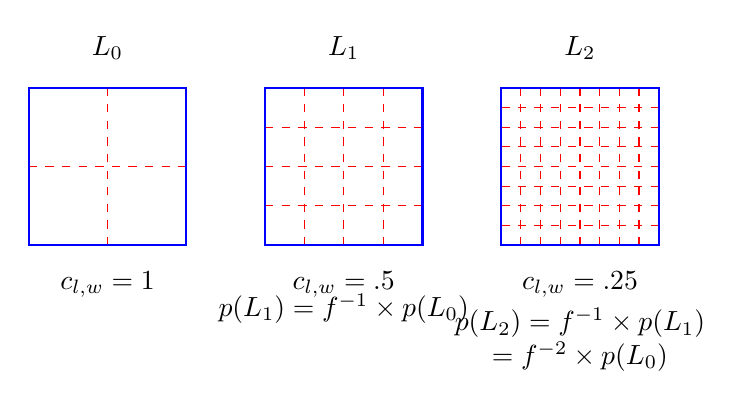
\begin{tikzpicture}
			\foreach \x/\step in {0/1,1/.5,2/.25} {
				\draw[red, dashed, step=\step] (3 * \x, 0) grid (3 * \x + 2, 2);
				\node at (1 + \x * 3, -.5) {\(c_{l,w}=\step\)};
			}
			\draw[blue, thick] (0,0) rectangle (2,2);
			\draw[blue, thick] (3,0) rectangle (5,2);
			\draw[blue, thick] (6,0) rectangle (8,2);
			
			\foreach \l/\cw in {0,1,2} {
				\node at (1 + \l * 3, 2.5) {\(L_{\l}\)};
			}
			
			\node at (4, -.8) {\(p(L_1)= f^{-1}\times p(L_0)\)};
			\node[align=center] at (7, -1.2) {\(p(L_2)= f^{-1} \times p(L_1)\)\\\(= f^{-2} \times p(L_0)\)};
		\end{tikzpicture}
	\end{figure}
	\subparagraph{Summary}
	To clear things up in this messy section full of variables it is helpful to take a look at table \ref{fig:messy_table}.
	\begin{figure}
		\centering
		\caption{Summary of all used variables}
		\label{fig:messy_table}
		\begin{tabular}{|l|p{.8\textwidth}|}
			\hline
			Variable        & Description \\ \hline
			\(c_{l,w},c_{l,h}\)  & The logic dimensions of a cluster define how many entries it has. All clusters have the same logical dimensions.\\ \hline
			\(c_{a,w},c_{a,h}\)  & The absolute dimensions of cluster define the size of the area the cluster covers. All clusters in the same level have the same absolute dimensions.\\ \hline
			\(p\)                & The precision is the distance two neighboring points in a cluster or level have.\\ \hline
			\(l_{l,w}, l_{l,h}\) & The logical dimension of a level define how many clusters it has. All levels have a different amount of clusters \\ \hline
			\(l_{a,w},l_{a,h}\)  & The absolute dimensions of a level define which area the level covers. All levels have the same absolute dimensions and position.     \\ \hline
		\end{tabular}
	\end{figure}
	\paragraph{Fractal Calculator}
	The calculator coordinates the calculation of values. The order to start is sent by the connector, alongside a list containing the clusters. As before mentioned values can only be calculated in bulk. The clusters provide a good 
	\subparagraph{Calculator Units}
	\paragraph{Image creation}
	\subsection{Internal Process Course}
	\section{Reflection}
	I would like to use this last section of my work to add my personal thoughts to my senior paper and to neatly close the discussion around my work.
	\subsection{Limitations, Bugs and Workarounds}
	Programs naturally come with hidden bugs and limitations. As my program became bigger more bugs to be squashed arose. I have due to time issues not been able to tackle every one and thus am obliged to shortly describe the bugs. One bug is also induced by factors outside of my range such as driver support.
	\paragraph{OpenCL on Macs}
	Apple decided to stop supporting OpenCL on its devices \cite{appleinsider}. Although the program detects the GPU and CPU as OpenCL devices, only the latter works.
	\paragraph{Magnification Limit}
	Every cluster \(C_i\) has an index \(i\) to store their location. This index is stored in a Java \verb|int| which can usually only assume values up to \(2^{64} - 1\). If the program tries to allocate a cluster with a higher index the program crashes due to a numerical overflow. This happens when \(l_{l,w} \times l_{l,h}\) is greater than the aforementioned value because \(i = a + b \times l_{l,w}\) where \(0 \leq a < l_{l,w}\) and \(0 \leq b < l_{l,h}\).\\
	If due to this it is no possible to render a specific area the following workaround is recommended: restart the application, but set the levels' position and dimension to the previously unavailable area.
	\paragraph{Memory Constraints}\label{sec:memory_problem}
	As the program calculates new values it stores them in RAM and VRAM, which both are limited in size. Without freeing any RAM during runtime the program is bound to try to allocate more RAM when no more is available, leading to a crash caused by an \verb|OutOfMemoryError|.
	\paragraph{Floating-Point precision}
	Floating point math on computers is if no special workarounds are used always tied to the machine precision, meaning that small rounding error occur during calculations. While the error is negligible on normally used numbers it can have devastating effects when the numbers become too small to be represented correctly. In my program this happens when the precision \(p\) becomes smaller than \(10^{-13}\), causing the values to be miscalculated.
	\subsection{Workflow}
	Programming an application of this size has come with many unexpected challenges which are tied to the nature of computer science. These challenges have, when not accounted for, caused either several delays in my time schedule or forced me to not implement a feature.
	\paragraph{Structure Design}
	The design as it is present now was the result of a long journey. At the very beginning it consisted of a simple program that calculated points of the Mandelbrot set, wrote the result into a file and then quit. It was all in just one file, without any logical structure. Because of the small size changes were easily introduced. However, new functionalities naturally increased the programs complexity by many times. The code was grouped in multiple modules which each took over a function. The advantage of modules is the ability to make internal changes to one without affecting other modules. This however does not hold true for any changes to the overall model, since this affects all modules. This happened quite often as I made many minor model changes due to having taken shortsighted decision, costing me much time. Another time stealing mistake of mine was the opposite: Thinking to big I made parts of the model more complex than they ultimately needed to be.\\
	An additional challenge was adding OpenCL functionality to my program. A major problem was that I had never before programmed in OpenCL and it was thus unknown territory for me. Another inconvenience was that the entire JVM crashed without any useful information if faulty parameters were passed to OpenCL functions. Since the debugger only works on Java code it was not possible to monitor such crashes with it, making the search for the solution quite cumbersome.
	\paragraph{Squashing bugs}
	One of the most banal and trivial hardships encountered are logical errors in the code, causing either simple misbehavior or runtime crashes. These can be prevented by using assertions. They are checks done at runtime to detect any illegal or senseless program states. If the check fails an \verb|AssertionError| is thrown to let the programmer know that there are issues in his code. I have used these extensively in combination with the OpenCL API.\\
	Assertions alone however are not enough. Sometimes it is useful to pause the execution and inspect the program state manually. This can be done by attaching a debugger to the running program. The debugger is able to pause the program execution at any moment and lets the programmer see the current state. It is also possible to set breakpoints, which cause the debugger to automatically pause execution when such a point is reached. Furthermore, it also pauses when an exception is about to be thrown. This was the most practical use for me since I was able to examine the cause leading to the exception.
	\subsection{Possible enhancements}\label{sec:poss_enh}
	The following sections shortly describe what features I would have added to my program if I have had any more time. Neither of them are crucial for my program but each of them would nonetheless bring more stability or comfort.
	\paragraph{OpenGL}
	Although the Java Swing Toolkit which is responsible for the GUI has longtime been replaced by newer alternatives I have decided to use it because it is the only type of GUI of which I am able to program. As of now, the image data has to be passed from OpenCL to the Java Swing application, resulting in a high latency and waste of resources. Had I had more time I would have made effort to implement an OpenGL GUI, which has features to work directly with OpenCL, saving valuable computing power. Another caveat is that since OpenCL works with native machine code it is more responsive and faster than the in any Java code.
	\paragraph{Memory to Disk}
	As mentioned in section \ref{sec:memory_problem}, the memory is a main cause of trouble when the application runs for long a duration. A possibility to combat this problem could be to offload unused data onto the disk, which as - in comparison to RAM - more than enough free space. The caveat here is to determine which data will probably not be used in the near future.
	\paragraph{Dynamic Iterations}
	A question left unanswered in my senior paper is the amount of iterations a point should go before it is considered part of the Mandelbrot set. The general rule of thumb is that the smaller the clip of the fractal is i.e. the closer the points to calculate are the more iterations are necessary to see a clear picture. In my program however the amount of iterations per point is indifferent to the distance between the points \(d\). Dynamically changing the maximal amount of iterations would drastically speed up the calculation of clips with a lower resolution and increase the quality of clips which have zoomed in greatly.\\
	This feature is already for the most part implemented in the program making it possible to give levels which are deeper more iterations. However I have not made any efforts to improve this feature because I simply lacked the time to investigate about how to determine the appropriate amount of iterations for a point.\\
	The default iteration model is named ``static'' and uses the same amount of iterations for every level. A not thoroughly tested variant named ``antiProportional'' can be selected in the settings, which increases the amount of iterations anti proportionally.
	\subsection{Conclusion}
	As described section \ref{sec:poss_enh} I was not able to implement every aspect I wanted to be included. However I can proudly present a program that meets all basic requirements I have given, such as being able to harness the power of a graphics card or exporting videos. Looking back at my work I can say that I made the mistake of investing too much time in the program and by far not enough in the paper.
	\clearpage
	\appendix
	\printbibliography
	
	
	
	
	
	
	
	
	
	
	
	
	
	
	
	
	
	
	
	
	
	
	
	%TODO
	\iffalse%Excludes rest of paper
	\section{OLD STUFF}
	\subsubsection{Image Generation}
	%take advantage of data arrangement, since sorted in clusters and levels and thus by precision
	%naive algorithm: search for nearest datapoint
	A less vital but still important aspect of my work is the visualization of the data. It is crucial to consider the way the data is stored when performing access-intense tasks, such as this. A more naive approach of mine search the whole dataset for each pixel colored, resulting in abysmal performance. By using a more sophisticated algorithm, the data can be directly mapped to the image without searching long for it. This section will go sequentially through all the steps taken.
	\paragraph{Image Parameters}
	\begin{figure}
		\centering
		\caption{Function Signature to create images}
		\label{fig:image_signature}
		\begin{verbatim}
		public Screen createScreen(int minPixelWidth, int minPixelHeight, Region region,
		                int threads, long maxWaitingTime)
		\end{verbatim}
	\end{figure}
	To know what type of image the program has to create, parameters have to be passed to the function called. As seen in figure \ref{fig:image_signature}, the first two refer to the (minimal) image constraints in pixels, \verb|region| describes the region of the fractal to render. \verb|threads| indicates the maximal, although not minimal, amount of CPU threads used to create the image, and \verb|maxWaitingTime| indicates how long the image creation can take before it is aborted to avoid blocking the application in case of an error, infinty loop or deadlock (although neither is likely to happen at all).\\
	The returned \verb|Screen| has at least the dimensions given by the parameters, but is very likely to surpass them. Due to the mapping of the pixels the actually displayed region might vary by at most a single pixel, but I have deemed that negligible.	
	\paragraph{Preparing the rendered Area}
	In figure \ref{fig:region_over_dataset}, the starting point of the problem is visible. A clip of the dataset has to be mapped onto the red region. Using the given dimensions of the red area, the necessary precision of the datapoints can be derived. Through the precision, we can calculate the necessary level and get the smallest logic region which can fit the red area inside it (figure \ref{fig:logic_region_over_dataset}). The logic region is needed to know from which level and place (index to be exact) in the dataset the data has to be queried, rending a long search for the datapoints redundant. The precision of the level is always better or equal to the precision of the requested image.	
	\begin{figure}
	\centering
	\caption{The dataset region(black) and the requested region (red)}
	\label{fig:region_over_dataset}
		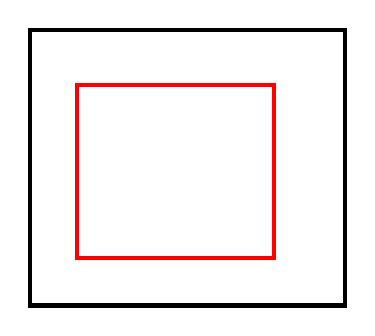
\begin{tikzpicture}
			\draw[ultra thick,black, step=.5] (0,0) rectangle (4,3.5);
			\draw[ultra thick,red] (0.6, .6) rectangle (3.1, 2.8);
		\end{tikzpicture}
	\end{figure}
	
	\begin{figure}
		\centering
		\caption{The level, its clusters and the logic region in green}
		\label{fig:logic_region_over_dataset}
		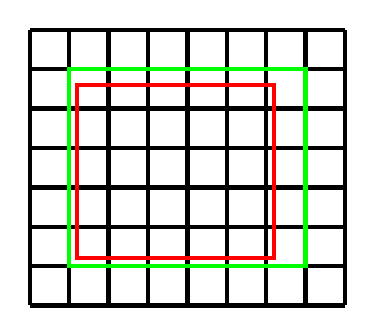
\begin{tikzpicture}
			\draw[ultra thick,black, step=.5] (0,0) grid (4, 3.5);
			\draw[ultra thick,red] (0.6, .6) rectangle (3.1, 2.8);
			\draw[ultra thick, green] (.5, .5) rectangle(3.5,3);
		\end{tikzpicture}
	\end{figure}
	\paragraph{Image allocation}
	Instead of allocating an empty image with the specified dimensions and filling it directly with data, the allocated image has the dimensions of the logical area. I have illustrated this in figure \ref{fig:logic_region_and_requested_area}. The logic cluster width and height are both 5, the logical area has the width and height of 3. The requested area lies unaligned with the rest in the middle, with a width of 5 and a height of 6. As seen in the image, the region where data is fetched from has a greater precision as the red requested area; The values in the dataset lie closer to each other than in the area.\\
	Following this example, the allocated image width is the logical cluster width times the logical region width (\(4 \times 5 = 20\)), and the image height is the logical cluster height times the logical area height (\(4 \times 6 = 24\)). The dimensions are measured in pixels. After it has been created, it can be immediately filled with data , which is a rather easy process since the pixels are by definition perfectly aligned with the data. In my program, this interim result is called \verb|ImageResult| and is cached for later usage(see section \ref{par:paragraph_image_creation_buffering}) \\
	After the image has been populated by the values, it can be cropped to the requested area. But as seen in figure \ref{fig:cropping the area}, the cropped image's properties are not as requested. The image is wider and taller than asked for, but this is a rather minor problem since it does not degrade the quality and can be easily corrected by scaling the image down. A bigger problem regarding the accuracy is that the returned clipping is slightly bigger than requested.
	
	\begin{figure}
		\centering
		\caption{The logical area (green) with clusters and values (blue), and the requested region (red) with pixels}
		\label{fig:logic_region_and_requested_area}
		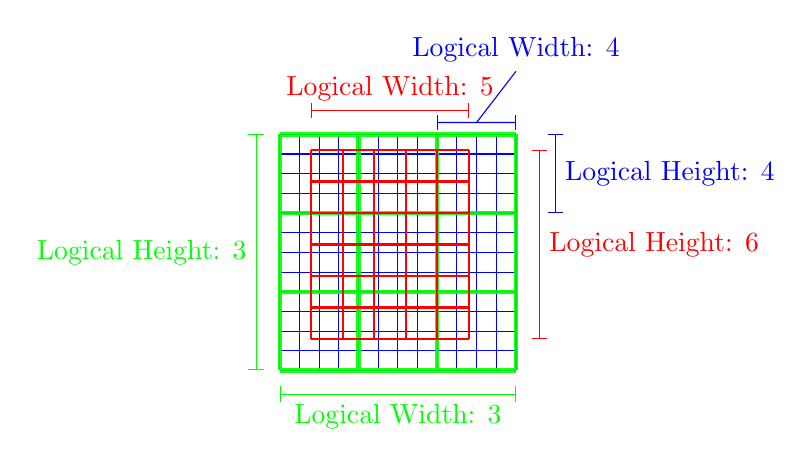
\begin{tikzpicture}
			\draw[|-|,green] (0, -.3) -- (1.5, -.3) node[below] {Logical Width: 3}-- (3, -.3);
			\draw[|-|,green] (-.3, 0) -- (-.3, 1.5) node[left] {Logical Height: 3}-- (-.3, 3);
			
			\draw[|-|,red] (0.4, 3.3) -- (1.4, 3.3) node[above] {Logical Width: 5}-- (2.4, 3.3);
			\draw[|-|,red] (3.3, 0.4)-- (3.3, 1.6) node[right] {Logical Height: 6}-- (3.3, 2.8);
			
			\draw[|-|,blue] (2, 3.15) -- (2.5, 3.15) -- (3, 3.8) node[above] {Logical Width: 4} -- (2.5,3.15)-- (3, 3.15);
			\draw[|-|,blue] (3.5, 2)-- (3.5, 2.5) node[right] {Logical Height: 4}-- (3.5, 3);
			
			\foreach \x in {0,1,2} {
				\foreach \y in {0,1,2} {
					\draw[blue, step=.25] (\x, \y) grid (\x +1, \y + 1);
				}
			};
			\draw[ultra thick, green, step=1, opacity=.9] (0, 0) grid (3,3);
			\draw[thick, red, step=.4] (0.4, 0.4) grid (0.4 + .4 * 5, 0.4 + .4 * 6);
		\end{tikzpicture}
	\end{figure}
	
	\begin{figure}
		\centering
		\caption{Cropping the image to the area given by the parameters}
		\label{fig:cropping the area}
		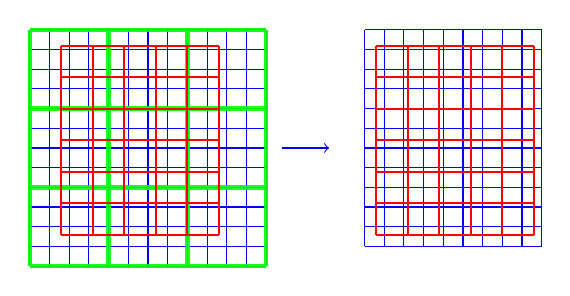
\begin{tikzpicture}			
		\foreach \x in {0,1,2} {
			\foreach \y in {0,1,2} {
				\draw[blue, step=.25] (\x, \y) grid (\x +1, \y + 1);
			}
		};
		\draw[ultra thick, green, step=1, opacity=.9] (0, 0) grid (3,3);
		\draw[thick, red, step=.4] (0.4, 0.4) grid (0.4 + .4 * 5, 0.4 + .4 * 6);
		
		\draw[->, blue] (3.2, 1.5) -- (3.8, 1.5);
		\draw[blue, step=.25] (4.24999, .25) grid (4 + 2.5, 3);
		\draw[thick, red, step=.4] (4.3999, 0.4) grid (4.4 + .4 * 5, 0.4 + .4 * 6);
		
		\end{tikzpicture}
	\end{figure}
	
	\paragraph{Buffering} \label{par:paragraph_image_creation_buffering}
	As mentioned above, generated \verb|ImageResult|s are cached for further usage. The reason becomes quite clear when thinking of the usual navigation in fractals. The user will often slowly zoom into a section of the set. This means for the render engine that it will create many images with a nearly identical area, thus being in the same logical area. Hence having a buffer filled with previously generated \verb|ImageResult|s can reduce the rendering time by much. Searching the buffer for a match takes place after knowing the logical area an image needs to be rendered. It is then checked against every entry in it, and if a suitable \verb|ImageResult| is found, it is taken and used instead of creating a new one from scratch. If this is not the case, a new \verb|ImageResult| has to strenuously be created and is afterwards added to the buffer.\\
	An issue encountered with buffering is the increasing RAM usage. Since the buffer contains only data which can be recreated at medium cost, it is not necessary to let it grow infinitely. Limiting its size leads to less RAM usage, but potentially a higher performance impact.\\ The buffer is only useful in cases where the roughly the same area is rendered often, such as zooming in or moving our a little. As soon as the area is moved around or zoomed in too much, thus requiring a new logical area or new depth respectively, a new \verb|ImageResult| has to be created.

	\fi
\end{document}